\documentclass{article}

\usepackage{arxiv}

\usepackage[utf8]{inputenc} % allow utf-8 input
\usepackage[T1]{fontenc}    % use 8-bit T1 fonts
\usepackage{lmodern}        % https://github.com/rstudio/rticles/issues/343
\usepackage{hyperref}       % hyperlinks
\usepackage{url}            % simple URL typesetting
\usepackage{booktabs}       % professional-quality tables
\usepackage{amsfonts}       % blackboard math symbols
\usepackage{nicefrac}       % compact symbols for 1/2, etc.
\usepackage{microtype}      % microtypography
\usepackage{lipsum}
\usepackage{graphicx}

\title{Evolution, functional diversity, regime shifts, hysteresis, and
nonlinearity; ecosystem responses to environmental change.}

\author{
    Owen L Petchey
   \\
    Department of Evolutionary Biology and Environmental Studies \\
    University of Zurich \\
  Zurich 8057, Switzerland \\
  \texttt{\href{mailto:owen.petchey@ieu.uzh.ch}{\nolinkurl{owen.petchey@ieu.uzh.ch}}} \\
   \And
    Rainer Krug
   \\
    Department of Evolutionary Biology and Environmental Studies \\
    University of Zurich \\
  Zurich 8057, Switzerland \\
  \texttt{\href{mailto:rainer.krug@ieu.uzh.ch}{\nolinkurl{rainer.krug@ieu.uzh.ch}}} \\
   \And
    Marcel Suleiman
   \\
    Department of Evolutionary Biology and Environmental Studies \\
    University of Zurich \\
  Zurich 8057, Switzerland \\
  \texttt{\href{mailto:marcel.suleiman@ieu.uzh.ch}{\nolinkurl{marcel.suleiman@ieu.uzh.ch}}} \\
  }


% Pandoc citation processing
\newlength{\csllabelwidth}
\setlength{\csllabelwidth}{3em}
\newlength{\cslhangindent}
\setlength{\cslhangindent}{1.5em}
% for Pandoc 2.8 to 2.10.1
\newenvironment{cslreferences}%
  {}%
  {\par}
% For Pandoc 2.11+
\newenvironment{CSLReferences}[3] % #1 hanging-ident, #2 entry spacing
 {% don't indent paragraphs
  \setlength{\parindent}{0pt}
  % turn on hanging indent if param 1 is 1
  \ifodd #1 \everypar{\setlength{\hangindent}{\cslhangindent}}\ignorespaces\fi
  % set entry spacing
  \ifnum #2 > 0
  \setlength{\parskip}{#2\baselineskip}
  \fi
 }%
 {}
\usepackage{calc} % for calculating minipage widths
\newcommand{\CSLBlock}[1]{#1\hfill\break}
\newcommand{\CSLLeftMargin}[1]{\parbox[t]{\csllabelwidth}{#1}}
\newcommand{\CSLRightInline}[1]{\parbox[t]{\linewidth - \csllabelwidth}{#1}}
\newcommand{\CSLIndent}[1]{\hspace{\cslhangindent}#1}



\begin{document}
\maketitle

\def\tightlist{}


\begin{abstract}
To be completed
\end{abstract}

\keywords{
    Biodiversity
   \and
    Evolution
   \and
    Hysteresis
   \and
    Alternate stable states
   \and
    Environmental change
   \and
    Regime shift
   \and
    Threshold
   \and
    Ecosystem
   \and
    Cyanobacteria
   \and
    Sulphur bacteria
  }

\hypertarget{introduction}{%
\section{Introduction}\label{introduction}}

Types of ecosystem responses to environmental change. What and why.
Importance of non-linearity and hysteresis. Feedbacks, diversity /
evolution. Includes graphical hypotheses. What is the relative
importance of feedbacks (composition) and diversity / evolution.

Ceulemans, R., Wojcik, L.A. \& Gaedke, U. (2021). Functional diversity
alters the effects of a pulse perturbation on the dynamics of tritrophic
food webs. \emph{bioRxiv}, 2021.03.22.436420.

(Dakos et al. 2019)

Anoxic-oxic ecosystem shifts as a case study. Contemporary relevance.
Intermediate complexity of system\ldots{} diagram of system, including
some panels of subsystems showing some of the positive feedbacks.
Central role of inhibition / tolerance. Also showing responses to
changes in oxygen diffusivity (justify from Bush et al this as a key
environmental driver).

Empirical evidence of variation in organismal tolerance. Across species
and evolution experiments. (Schoeffler et al. 2019)

Recent experimental evolution studies have demonstrated considerable
increases in tolerance. For example, the sulphur bacteria
\emph{Desulfovibrio vulgaris} evolved a 32-fold increase in oxygen
tolerance (Schoeffler et al. 2019) . Furthermore, the evolved strains
were capable of oxygen respiration that permits growth. Genome
re-sequencing revealed that few mutations were involved. Additionally,
the cyanobacterium \emph{Microcystis aeruginosa} evolved a four-fold
higher sulphide tolerance via rare spontaneous mutations
(Martín-Clemente et al. 2019). In that study, populations with higher
genetic variation and those experiencing slower environmental change (an
increase in sulphide concentration) were more likely to persist at high
sulphide concentration.

(Rolfe et al. 1978) - Factors related to the oxygen tolerance of
anaerobic bacteria. (Ramel et al. 2015) - ``they were able to grow but
the final biomasses and the growth yield were lower than that obtained
under anaerobic conditions,'' ``Determination of the molar growth yields
on lactate suggested that a part of the energy gained from lactate
oxidation was derived toward cells protection/repairing against
oxidative conditions rather than biosynthesis'' (Hamilton et al. 2018) -
``Cyanobacterial photosynthesis under sulfidic conditions: insights from
the isolate Leptolyngbya sp. strain hensonii''

Physiological tolerances to environmental conditions, including
interspecific variation in tolerance and evolution of tolerance, are a
key component of the engineering of ecosystem for determining their
stability (Minervini \emph{et al.} 2014)(Gómez‐Gras \emph{et al.}
2019)(Cuenca Cambronero \emph{et al.} 2018)(Vos \emph{et al.}
2017)(Evans \& Wallenstein 2014)(Rolfe \emph{et al.} 1978)(Knoll \&
Bauld 1989)(Girvan \emph{et al.} 2005).

Questions: - How does variation organismal tolerances affect response

Approach: - Modelling the system with ODEs. - Diversity manipulation
(can be considered selection among strains, or selection among species).
- Do not include mutation.

\hypertarget{methods}{%
\section{Methods}\label{methods}}

\hypertarget{the-model}{%
\subsection{The model}\label{the-model}}

Bush et al (2017) contains an excellent description of the model of the
ecosystem. Here we only describe the extensions needed for modelling
multiple strains/taxa per functional group.

\hypertarget{measurement-of-non-linearity-and-hysteresis}{%
\subsection{Measurement of non-linearity and
hysteresis}\label{measurement-of-non-linearity-and-hysteresis}}

Take from Garnier et al.

Rate-independent hysteresis, because we are considering only stable
states, and not rate-dependent hysteresis, which can occur when a lag in
the system response to an environmental response causes a difference
between the observed system state at time \(t\) and the stable state for
the environmental conditions present at time \(t\).

\hypertarget{implementation}{%
\subsection{Implementation}\label{implementation}}

R package.

\hypertarget{results}{%
\section{Results}\label{results}}

\hypertarget{figure-stable-states-with-and-without-variation.}{%
\subsection{Figure: Stable states with and without
variation.}\label{figure-stable-states-with-and-without-variation.}}

\begin{figure}

{\centering 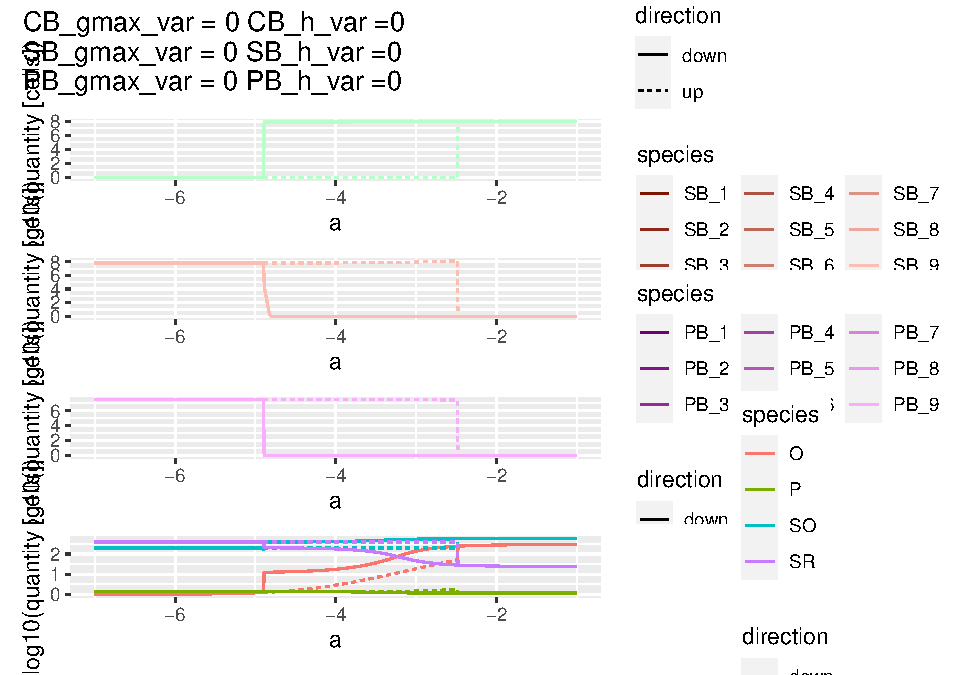
\includegraphics[width=1\linewidth]{article_files/figure-latex/ss_novar-1} 

}

\caption{your caption}\label{fig:ss_novar}
\end{figure}

`

\begin{figure}

{\centering 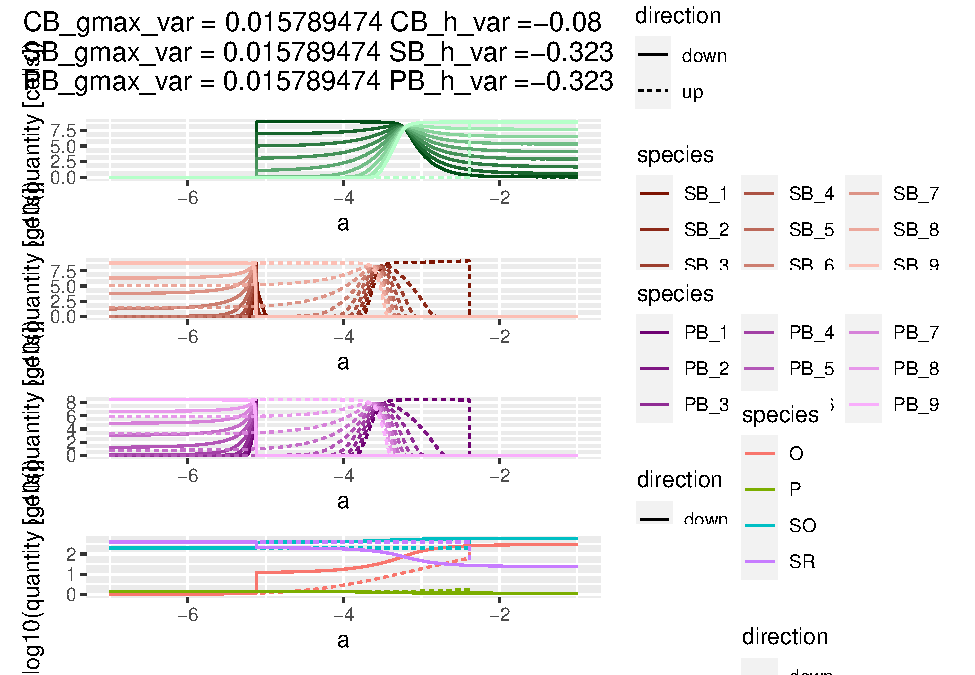
\includegraphics[width=1\linewidth]{article_files/figure-latex/ss_var-1} 

}

\caption{your caption}\label{fig:ss_var}
\end{figure}

\begin{figure}

{\centering \includegraphics[width=1\linewidth]{article_files/figure-latex/ss_var2-1} 

}

\caption{your caption}\label{fig:ss_var2}
\end{figure}

\hypertarget{figure-hysteresis-shift-point-nonlinearity-as-var-increases.}{%
\subsection{Figure: hysteresis, shift point, nonlinearity, as var
increases.}\label{figure-hysteresis-shift-point-nonlinearity-as-var-increases.}}

\begin{figure}

{\centering \includegraphics[width=1\linewidth]{article_files/figure-latex/ss_var3-1} 

}

\caption{your caption}\label{fig:ss_var3}
\end{figure}

\hypertarget{figure-temporal-switches}{%
\subsection{Figure: Temporal switches}\label{figure-temporal-switches}}

To be added. Need to go both ways (oxic to anoxic, and anoxic to oxic).

\hypertarget{discussion}{%
\section{Discussion}\label{discussion}}

\url{https://onlinelibrary.wiley.com/doi/10.1111/gcb.15662?af=R}

\url{https://onlinelibrary.wiley.com/doi/10.1111/ele.13760?af=R}

\hypertarget{acknowledgements}{%
\section{Acknowledgements}\label{acknowledgements}}

SNF URPP

\hypertarget{refs}{}
\begin{CSLReferences}{1}{0}
\leavevmode\hypertarget{ref-dakos2019}{}%
Dakos, Vasilis, Blake Matthews, Andrew P. Hendry, Jonathan Levine,
Nicolas Loeuille, Jon Norberg, Patrik Nosil, Marten Scheffer, and Luc De
Meester. 2019. {``Ecosystem Tipping Points in an Evolving World.''}
\emph{Nature Ecology \& Evolution} 3 (3): 355--62.
\url{https://doi.org/10.1038/s41559-019-0797-2}.

\leavevmode\hypertarget{ref-hamilton2018}{}%
Hamilton, Trinity L., Judith M. Klatt, Dirk de Beer, and Jennifer L.
Macalady. 2018. {``Cyanobacterial Photosynthesis Under Sulfidic
Conditions: Insights from the Isolate Leptolyngbya Sp. Strain
Hensonii.''} \emph{The ISME Journal} 12 (2): 568--84.
\url{https://doi.org/10.1038/ismej.2017.193}.

\leavevmode\hypertarget{ref-martuxednclemente2019}{}%
Martín-Clemente, Elena, Ignacio J. Melero-Jiménez, Elena Bañares-España,
Antonio Flores-Moya, and María J. García-Sánchez. 2019. {``Adaptation
Dynamics and Evolutionary Rescue Under Sulfide Selection in
Cyanobacteria: A Comparative Study Between {\emph{Microcystis
Aeruginosa}} and {\emph{Oscillatoria}} Sp. (Cyanobacteria).''}
\emph{Journal of Phycology} 55 (6): 1348--60.
\url{https://doi.org/10.1111/jpy.12911}.

\leavevmode\hypertarget{ref-ramel2015}{}%
Ramel, Fanny, Gael Brasseur, Laetitia Pieulle, Odile Valette, Agnès
Hirschler-Réa, Marie Laure Fardeau, and Alain Dolla. 2015. {``Growth of
the Obligate Anaerobe Desulfovibrio Vulgaris Hildenborough Under
Continuous Low Oxygen Concentration Sparging: Impact of the
Membrane-Bound Oxygen Reductases.''} \emph{PLOS ONE} 10 (4): e0123455.
\url{https://doi.org/10.1371/journal.pone.0123455}.

\leavevmode\hypertarget{ref-rolfe1978}{}%
Rolfe, Rial D., David J. Hentges, Benedict J. Campbell, and James T.
Barrett. 1978. {``Factors Related to the Oxygen Tolerance of Anaerobic
Bacteria.''} \emph{Applied and Environmental Microbiology} 36 (2):
306--13. \url{https://www.ncbi.nlm.nih.gov/pmc/articles/PMC291219/}.

\leavevmode\hypertarget{ref-schoeffler2019}{}%
Schoeffler, Marine, Anne-Laure Gaudin, Fanny Ramel, Odile Valette, Yann
Denis, Wagdi Ben Hania, Agnès Hirschler-Réa, and Alain Dolla. 2019.
{``Growth of an Anaerobic Sulfate-Reducing Bacterium Sustained by Oxygen
Respiratory Energy Conservation After O {\textsubscript{2}} -Driven
Experimental Evolution: O {\textsubscript{2}} -Driven Experimental
Evolution of {\emph{Desulfovibrio}}.''} \emph{Environmental
Microbiology} 21 (1): 360--73.
\url{https://doi.org/10.1111/1462-2920.14466}.

\end{CSLReferences}

\bibliographystyle{unsrt}
\bibliography{references.bib}


\end{document}
